\documentclass[11pt]{article}
\usepackage[textwidth=18.0cm, textheight=23.0cm, top=2.0cm]{geometry}
\usepackage{pst-all}
\usepackage{amssymb}
\usepackage{tikz}
\usepackage{underscore}\begin{document}
\pagestyle{empty}


ClassName: \underline{\textbf{Class_10.2bp-1}}
\par
BinSize: \underline{\textbf{100 × 100}}
\par
ReduceSize: \underline{\textbf{100 × 100}}
\par
TypeNum: \underline{\textbf{20}}
\par
Num: \underline{\textbf{20}}
\par
OutS: \underline{\textbf{30000}}
\par
InS: \underline{\textbf{23581}}
\par
Rate: \underline{\textbf{0.786}}
\par
UB: \underline{\textbf{3}}
\par
LB0: \underline{\textbf{3}}
\par
LB: \underline{\textbf{3}}
\par
LBWithCut: \underline{\textbf{3}}
\par
NodeCut: \underline{\textbf{0}}
\par
ExtendedNodeCnt: \underline{\textbf{1}}
\par
GenNodeCnt: \underline{\textbf{1}}
\par
PrimalNode: \underline{\textbf{0}}
\par
ColumnCount: \underline{\textbf{3}}
\par
TotalCutCount: \underline{\textbf{0}}
\par
RootCutCount: \underline{\textbf{0}}
\par
LPSolverCnt: \underline{\textbf{1}}
\par
PricingSolverCnt: \underline{\textbf{0}}
\par
BranchAndBoundNum: \underline{\textbf{1}}
\par
isOpt: \underline{\textbf{true}}
\par
TimeOnInitSolution: \underline{\textbf{600.000 s}}
\par
TimeOnPrimal: \underline{\textbf{0.000 s}}
\par
TimeOnPricing: \underline{\textbf{0.000 s}}
\par
TimeOnRmp: \underline{\textbf{0.046 s}}
\par
TotalTime: \underline{\textbf{600.281 s}}
\par
\newpage


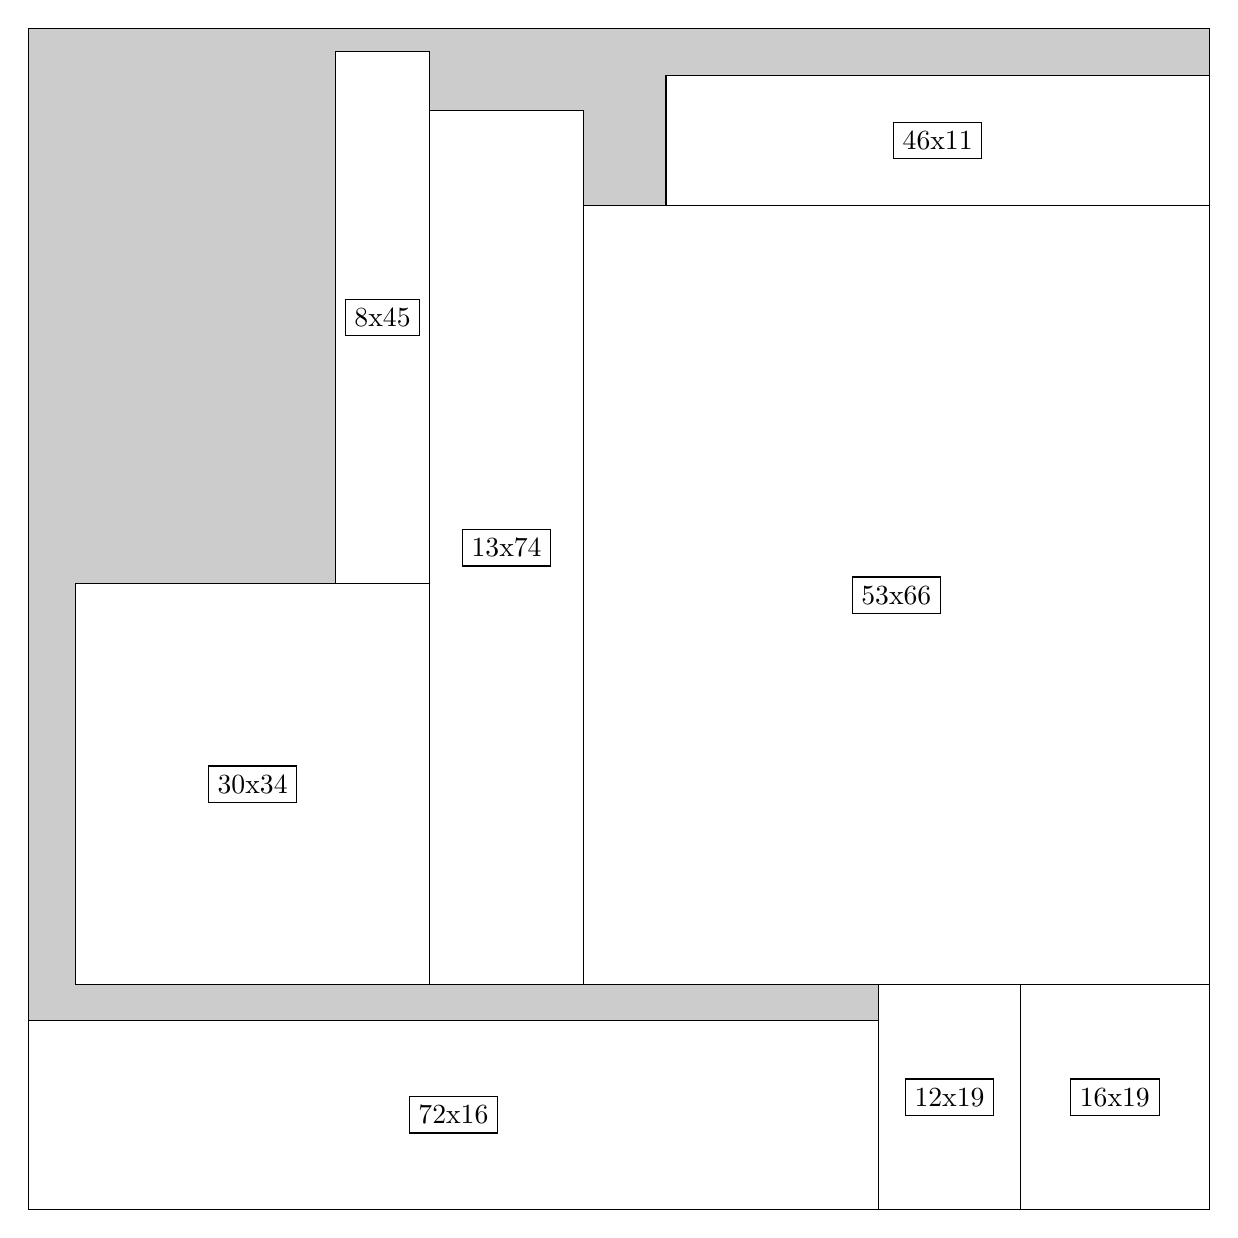
\begin{tikzpicture}[shorten >=1pt,scale=1.0,every node/.style={scale=1.0},->]
\tikzstyle{vertex}=[circle,fill=black!25,minimum size=14pt,inner sep=0pt]
\filldraw[fill=gray!40!white, draw=black] (0,0) rectangle (15.0,15.0);
\foreach \name/\x/\y/\w/\h in {16x19/12.6/0.0/2.4/2.85,12x19/10.799999999999999/0.0/1.7999999999999998/2.85,72x16/0.0/0.0/10.799999999999999/2.4,53x66/7.05/2.85/7.949999999999999/9.9,46x11/8.1/12.75/6.8999999999999995/1.65,13x74/5.1/2.85/1.95/11.1,30x34/0.6/2.85/4.5/5.1,8x45/3.9/7.949999999999999/1.2/6.75}
\filldraw[fill=white!40!white, draw=black] (\x,\y) rectangle node[draw] (\name) {\name} ++(\w,\h);
\end{tikzpicture}


w =16 , h =19 , x =84 , y =0 , v =304
\par
w =12 , h =19 , x =72 , y =0 , v =228
\par
w =72 , h =16 , x =0 , y =0 , v =1152
\par
w =53 , h =66 , x =47 , y =19 , v =3498
\par
w =46 , h =11 , x =54 , y =85 , v =506
\par
w =13 , h =74 , x =34 , y =19 , v =962
\par
w =30 , h =34 , x =4 , y =19 , v =1020
\par
w =8 , h =45 , x =26 , y =53 , v =360
\par
\newpage


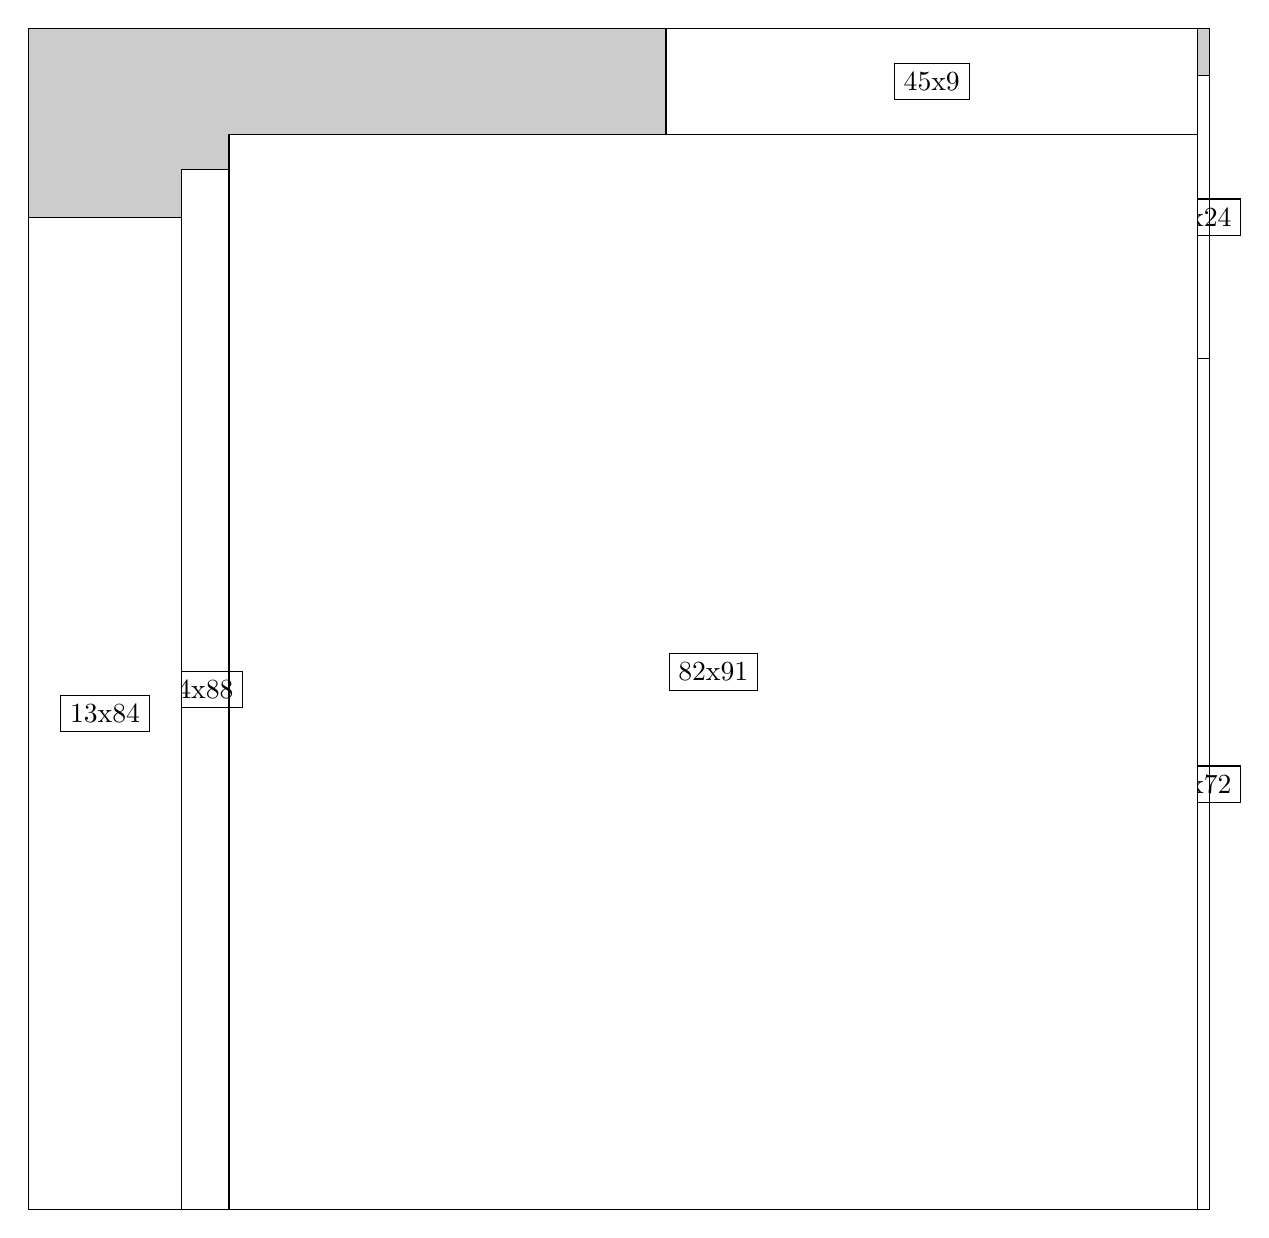
\begin{tikzpicture}[shorten >=1pt,scale=1.0,every node/.style={scale=1.0},->]
\tikzstyle{vertex}=[circle,fill=black!25,minimum size=14pt,inner sep=0pt]
\filldraw[fill=gray!40!white, draw=black] (0,0) rectangle (15.0,15.0);
\foreach \name/\x/\y/\w/\h in {1x72/14.85/0.0/0.15/10.799999999999999,1x24/14.85/10.799999999999999/0.15/3.5999999999999996,82x91/2.55/0.0/12.299999999999999/13.65,45x9/8.1/13.65/6.75/1.3499999999999999,4x88/1.95/0.0/0.6/13.2,13x84/0.0/0.0/1.95/12.6}
\filldraw[fill=white!40!white, draw=black] (\x,\y) rectangle node[draw] (\name) {\name} ++(\w,\h);
\end{tikzpicture}


w =1 , h =72 , x =99 , y =0 , v =72
\par
w =1 , h =24 , x =99 , y =72 , v =24
\par
w =82 , h =91 , x =17 , y =0 , v =7462
\par
w =45 , h =9 , x =54 , y =91 , v =405
\par
w =4 , h =88 , x =13 , y =0 , v =352
\par
w =13 , h =84 , x =0 , y =0 , v =1092
\par
\newpage


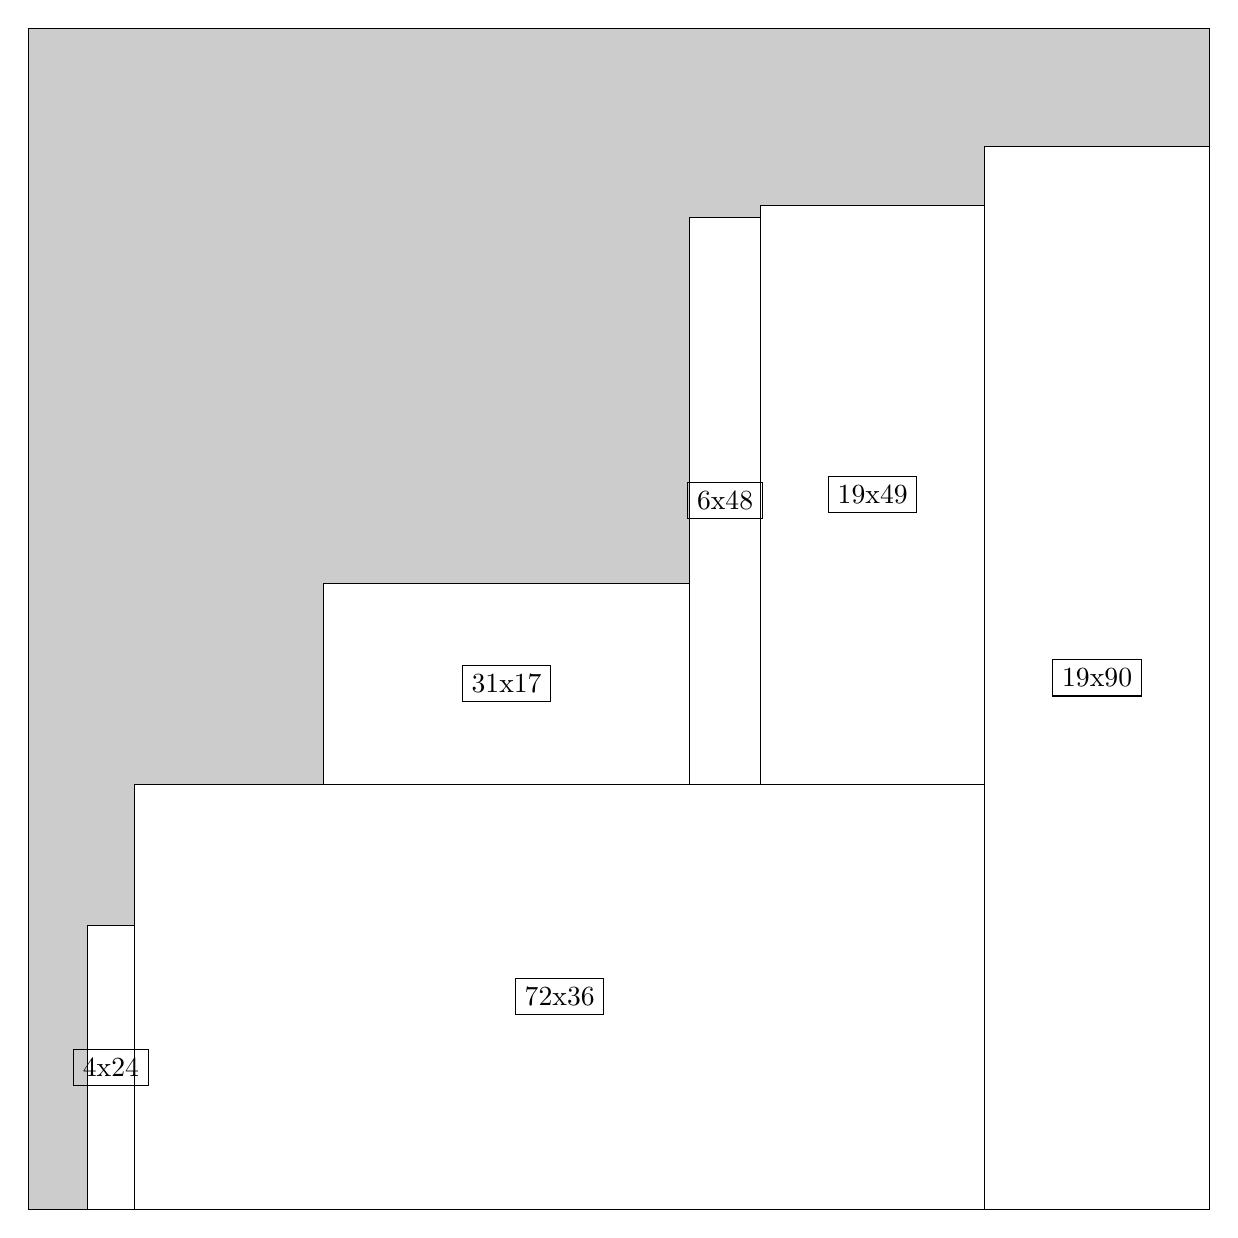
\begin{tikzpicture}[shorten >=1pt,scale=1.0,every node/.style={scale=1.0},->]
\tikzstyle{vertex}=[circle,fill=black!25,minimum size=14pt,inner sep=0pt]
\filldraw[fill=gray!40!white, draw=black] (0,0) rectangle (15.0,15.0);
\foreach \name/\x/\y/\w/\h in {19x90/12.15/0.0/2.85/13.5,72x36/1.3499999999999999/0.0/10.799999999999999/5.3999999999999995,4x24/0.75/0.0/0.6/3.5999999999999996,19x49/9.299999999999999/5.3999999999999995/2.85/7.35,6x48/8.4/5.3999999999999995/0.8999999999999999/7.199999999999999,31x17/3.75/5.3999999999999995/4.6499999999999995/2.55}
\filldraw[fill=white!40!white, draw=black] (\x,\y) rectangle node[draw] (\name) {\name} ++(\w,\h);
\end{tikzpicture}


w =19 , h =90 , x =81 , y =0 , v =1710
\par
w =72 , h =36 , x =9 , y =0 , v =2592
\par
w =4 , h =24 , x =5 , y =0 , v =96
\par
w =19 , h =49 , x =62 , y =36 , v =931
\par
w =6 , h =48 , x =56 , y =36 , v =288
\par
w =31 , h =17 , x =25 , y =36 , v =527
\par
\newpage


\end{document}